本プラットフォーム上で,教材提供者は過去のアプリケーションを用いたい場合がある.
それに対応するため,教材提供者がDockerを用いて作成したアプリケーションを本プラットフォームでも利用可能にするためコンテナ管理機能を作成した.
本機能を利用するには,本プラットフォームで動作させたいコンテナ情報が記載されたDockerfileとdocker-compose.ymlを事前にGithubなどのリポジトリに用意する.
外部通信が必要なアプリケーションの場合,本機能が提示するポート番号のみが利用可能となっている.
以上の情報を,本機能が提示するフォームに入力することにより,本プラットフォームでDockerのコンテナを作成し,アクセスするためのURLが画面上に表示される.
教材提供者は発行されたURLにアクセスすることで動作を確認できる.
また,発行された URL をコンテンツ提供機能の本文に貼り付けることにより,学習者はそのコンテンツを利用できる.

本機能の入力画面と入力が完了し,コンテナが作成された後の画面を図\ref{container_ex_before},図\ref{container_ex_after}に示す.

\begin{figure}[htbp]
    \begin{center}
        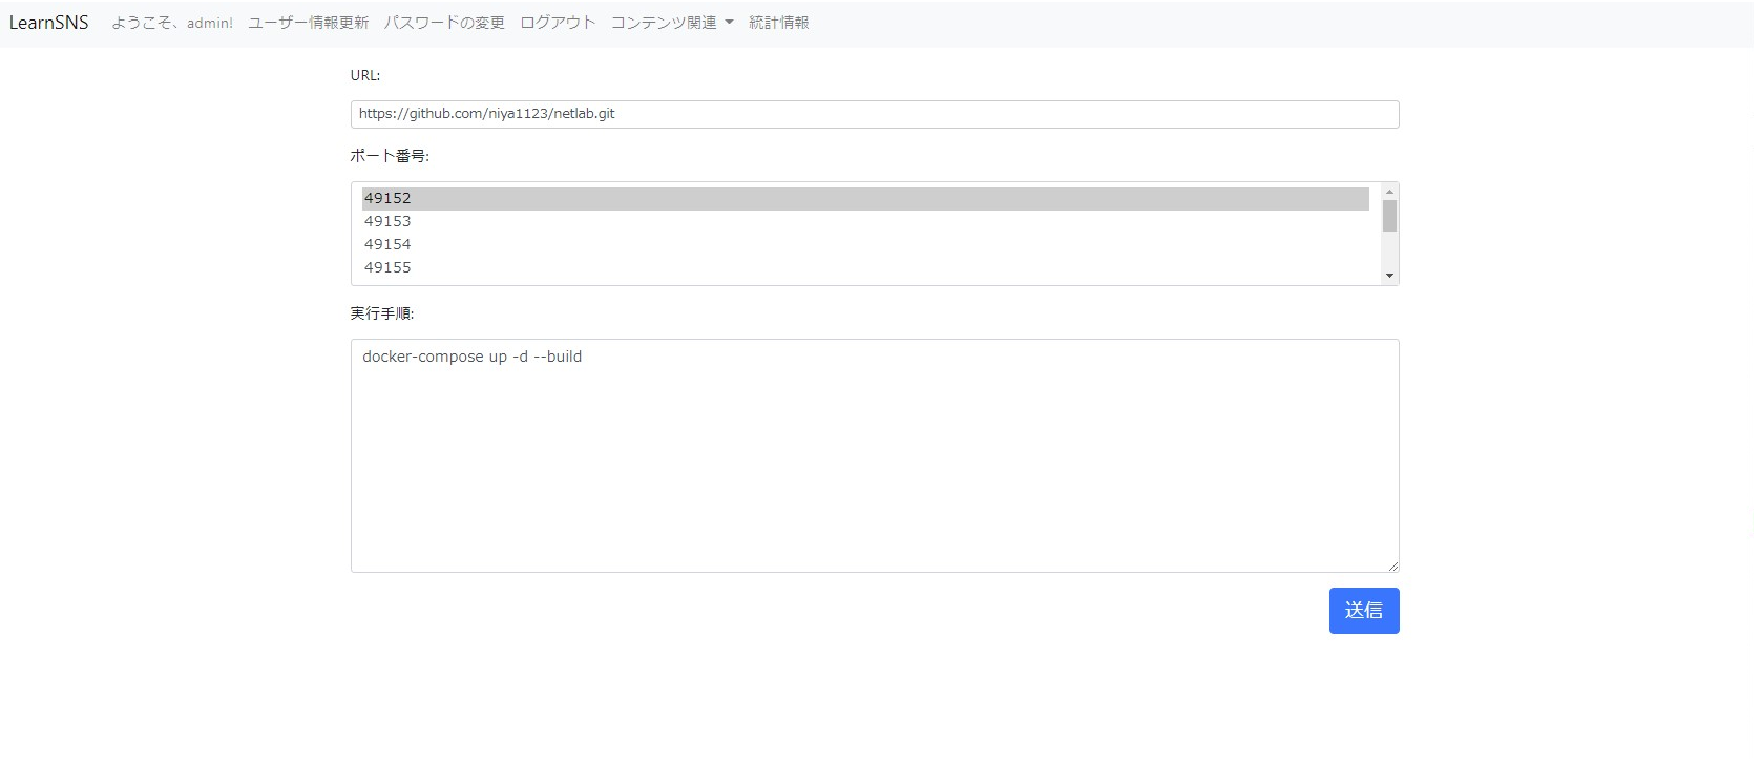
\includegraphics[width=18cm,height=17cm,keepaspectratio]{container_before-crop.pdf}\\
        %includegraphicsの詳しい使い方ははLaTeXの参考書を参照.
    \end{center}
    \caption{コンテナ管理機能の入力画面}
    \label{container_ex_before}
\end{figure}

\begin{figure}[htbp]
    \begin{center}
        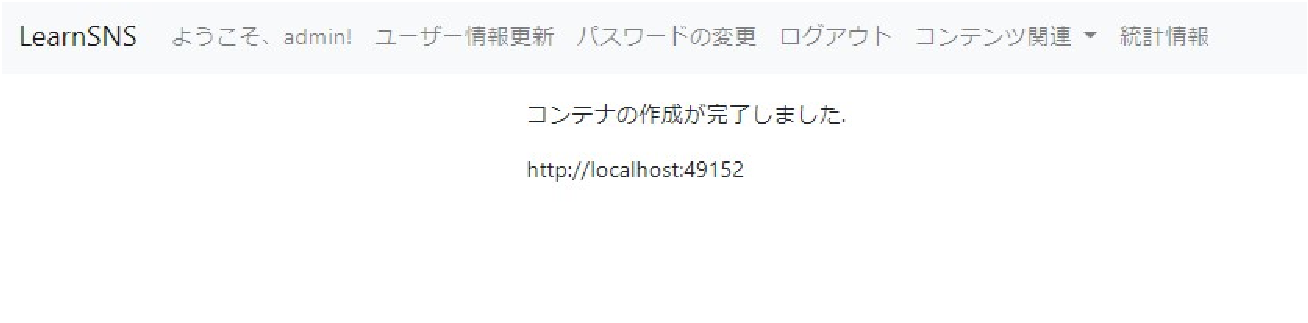
\includegraphics[width=13cm,height=12cm,keepaspectratio]{container_after-crop.pdf}\\
        %includegraphicsの詳しい使い方ははLaTeXの参考書を参照.
    \end{center}
    \caption{コンテナ管理機能のコンテナ作成後の画面}
    \label{container_ex_after}
\end{figure}

